\section{Deployment diagram}
\vspace{0.5cm}

\begin{figure}[H]
    \centering
    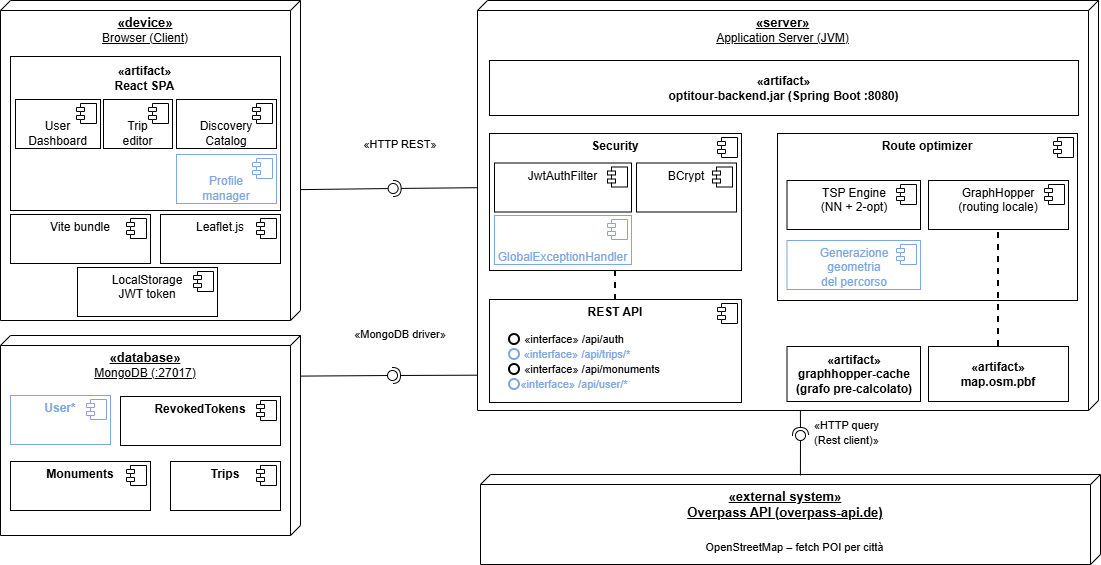
\includegraphics[width=0.85\textwidth]{Iterazione3/Diagrammi/DeploymentDiagram3.png}
    \caption{Diagramma di deployment}
    \label{fig:class_deploymentdiagram3}
\end{figure}

A seguito delle funzionalità aggiunte a livello di codice, il diagramma di deployment ha subito le seguenti variazioni:

\begin{itemize}
    \item \textbf{Gestione Profilo Utente:} Implementazione di una gestione completa del profilo.
    \begin{itemize}
        \item \textbf{Gestione Dati:} Introduzione di endpoint (\texttt{PATCH /api/user/profile}) per la modifica delle credenziali.
        \item \textbf{Eliminazione Account:} Funzionalità di rimozione definitiva (\texttt{DELETE /api/user/profile}) con rimozione a cascata delle entità correlate.
        \item \textbf{Interfaccia Frontend:} Nuova sezione dedicata per la visualizzazione e modifica dei dati personali.
    \end{itemize}

    \item \textbf{Funzionalità Avanzate per i Viaggi:} Arricchimento del modulo viaggi per migliorarne la riusabilità.
    \begin{itemize}
        \item \textbf{Esportazione PDF:} Implementazione dell'endpoint \texttt{GET /api/trips/\{id\}/export}.
    \end{itemize}

    \item \textbf{Ottimizzazione e Visualizzazione Percorso:} Evoluzione del motore \texttt{OptimizationEngine}.
    \begin{itemize}
        \item \textbf{Integrazione GraphHopper:} Logica di calcolo del percorso basata su strade pedonali reali.
        \item \textbf{Geometria del Percorso:} Il metodo \texttt{getRouteLeg} recupera la polilinea del percorso; in caso di assenza del servizio, viene applicato un \textit{fallback} lineare.
        \item \textbf{Risultato:} Aggiornamento dell'oggetto \texttt{TspResult} per includere la geometria dettagliata, permettendo al frontend il rendering delle tratte reali.
    \end{itemize}

    \item \textbf{Security:} Implementazione del componente \texttt{GlobalExceptionHandler}.
    \begin{itemize}
        \item Si tratta di una classe \texttt{@RestControllerAdvice} che intercetta globalmente le eccezioni, traducendole in risposte HTTP semanticamente corrette (es. \texttt{409 Conflict} per dati duplicati, \texttt{404 Not Found} per risorse inesistenti).
    \end{itemize}
\end{itemize}